\documentclass[xcolor=svgnames,dvipsnames,table, hyperref=pdftex, mathserif, presentation]{beamer}
\usepackage{amsmath,amssymb,amsfonts,amsthm}
\usepackage{ctex}
\setCJKsansfont{KaiTi}% 文泉驿的黑体
\usepackage{graphics}
\usepackage{graphicx}
\usepackage{xcolor}
\usepackage{wasysym}
\usepackage{bbm}
\usepackage{url}
\usepackage{beamerleanprogress}
\usepackage{tikz-dependency}
\usepackage{tikz-qtree}
\usepackage{multirow}

% for uml charts
\usepackage{tikz}
\usetikzlibrary{calc,arrows.meta, graphs, trees, shapes, positioning, automata,
shapes.geometric, shapes.multipart, er, patterns, decorations.markings, intersections, decorations.text}
\usepackage{tikz-uml}

% for overlap pictures
\usepackage{overpic}

% for customize itemize
% \usepackage{lipsum}
% \usepackage{paralist}
% \setbeamertemplate{itemize/enumerate body begin}{\large}
% \setbeamertemplate{itemize/enumerate subbody begin}{\tiny}


\newcommand{\tabincell}[2]{\begin{tabular}{@{}#1@{}}#2\end{tabular}}%放在导言区
\usetheme{CambridgeUS}
%\usetheme{Pittsburgh}
\usecolortheme{orchid} % seahorse  orchid rose
\setbeamertemplate{blocks}[rounded][shadow=true]
\AtBeginSection[]{%
  \begin{frame}<beamer>
    \frametitle{Outline}
      \tableofcontents[current] 
    \end{frame}
  \addtocounter{framenumber}{-1}% If you don't want them to affect the slide number
}
\AtBeginSubsection[]
{
  \begin{frame}
  \frametitle{Outline}
    \tableofcontents[currentsection,currentsubsection]
  %\tableofcontents[sectionstyle=show/hide,subsectionstyle=hide/show/hide]
  \end{frame}
  \addtocounter{framenumber}{-1}% If you don't want them to affect the slide number
}
\newcommand{\setof}[1]{\ensuremath{\left \{ #1 \right \}}}
\newcommand{\tuple}[1]{\ensuremath{\left \langle #1 \right \rangle }}
\newcommand{\red}[1]{\textcolor{red}{#1}}
\newcommand{\brown}[1]{\textcolor{brown}{#1}}
\newcommand{\green}[1]{\textcolor{green}{#1}}
\newcommand{\blue}[1]{\textcolor{blue}{#1}}
\newcommand{\cyan}[1]{\textcolor{cyan}{#1}}

%gets rid of navigation symbols
\setbeamertemplate{navigation symbols}{}

\begin{document}
 
\title[2015春总结]{Knowledge Base Unification via Sense Embeddings and Disambiguation}

\institute[icst@pku]{
  icst-wip
}
\author[Zhe Han]{\\ 
Claudio Delli Bovi @uniroma1 \begin{footnotesize}罗马大学\end{footnotesize}\\
Luis Espinosa-Anke @upf \begin{footnotesize}庞培法布拉大学\end{footnotesize}\\
Roberto Navigli @uniroma1\\
}

\frame[t,plain]{ \titlepage } % [t,plain]

\frame{
  \frametitle{ Outline  }
  
   \begin{itemize}
    \item summary
      \begin{itemize}
       \item 问题、方法概述
       \item 相关工作
       \item 实验使用的工具
      \end{itemize}
    \item 归一化(Unification)的方法
      \begin{itemize}
       \item 实体消歧(entity disambiguation)
       \item 关系对应(relation alignment)
      \end{itemize}
    \item 实验

   \end{itemize}

}


\frame{
  \frametitle{summary/author}
  \begin{figure}[h]
      \begin{overpic}[scale=.4]
	{pic/navigli.jpg}
      \end{overpic}
      \begin{overpic}[scale=.4]
	{pic/claudio.jpg}
	\only<2>{\put(-1,0){
	  \setlength{\fboxrule}{3pt} 
	  \setlength{\fboxsep}{0cm} 
	  \fbox{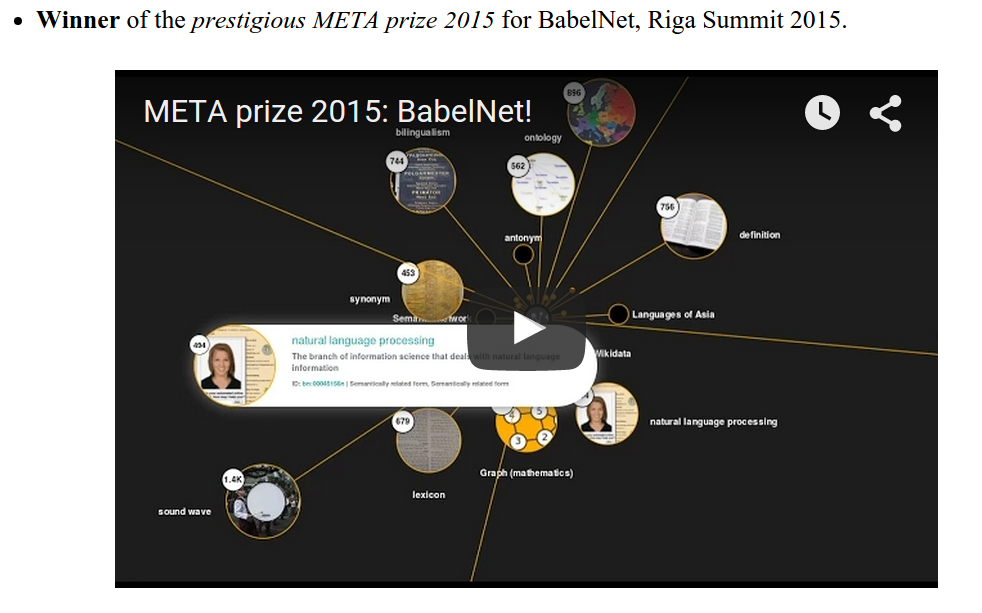
\includegraphics[width=0.5\hsize]{pic/navigli-babelNet.png}} 
	}}
      \end{overpic}
  \end{figure}

  \begin{itemize}
   \item Claudio Delli Bovi
    \begin{itemize}
     \item 罗马大学博士,计算语言学方向,主要研究语法、句法结构,目前在做WSD
    \end{itemize}
   \item Roberto Navigli
    \begin{itemize}
     \item Claudio的导师,07年博士毕业,BabelNet/Babelfy
    \end{itemize}

  \end{itemize}

}
\frame{
  \frametitle{\only<1-2>{summary/motivation}\only<3->{summary/method}}
  \begin{columns}
  \column{0.99\hsize}
      \begin{footnotesize}
  \begin{tikzpicture}
    \tikzstyle{Node}=[draw, rectangle, rounded corners, align=center]
    \node [Node, text width=2.5cm] (entity) {
      \emph{实体} \\ 
      \begin{footnotesize}
      \red{李娜(网球运动员)} \\ 
      \red{ 李娜(歌手)}\\
      \red{李娜(游泳运动员)}\\
      \red{姜山(网球运动员)}\\
      \red{张家辉 \\ ...}\\
      \end{footnotesize}
    };
    \node [Node, text width=1.5cm, right=of entity] (type) {
      \emph{关系} \\ 
      \begin{footnotesize}
      \brown{配偶}\\
      \brown{出生日期}\\
      \brown{子女\\ ...}\\
      \end{footnotesize}
    };
    \only<5>{
    \node [Node, text width=3cm, right=of type] (exap1) {
      【一】\\
      \begin{footnotesize}
      \blue{微软-CEO-纳德拉}
      \blue{搜狐-CEO-张朝阳}\\
      \blue{\red{苹果(?)}-CEO-库克}\\
      ...
      \end{footnotesize}
    };
    }
    \only<6>{
    \node [Node, text width=3cm, right=of type] (exap1) {
      【二】\\
      \begin{footnotesize}
      \blue{花果山-所在-连云港}\\ 
      \blue{全国政协-所在-北京}\\ 
      \blue{\red{大众}-所在-黑龙江} (这里指大众乡)
      ...
      \end{footnotesize}
    };
    }
    \node [Node, text width=3.5cm, below=of entity] (tripleWP) {
      zh.wikipedia:李娜-丈夫-姜山
    };
    \node [Node, text width=4cm, below=of tripleWP] (tripleNew) {
      \begin{footnotesize}
      \red{李娜(网球运动员)}-\brown{配偶}-\red{姜山}
      \end{footnotesize}
    };
    \node [Node, text width=3.5cm, below=of tripleNew] (tripleHD) {
      zh.hudong:李娜(网球)-夫婿-姜山(湖北人)
    };
    \node [Node, text width=7.05cm, right=of tripleNew] (desc) {
   \only<1>{
    \begin{large}
     如何整合多个知识库?\\
    \end{large}
    \begin{itemize}\begin{footnotesize}
     \item 全部在subject-predicate-object数据库上
     \item 知识库可能是完全非结构化的(主语只是普通字符串)
     \item 给定一个标准的数据库(左上的实体+关系)
     \item 其他的数据库可能存在歧义,结构不标准
     \end{footnotesize}
    \end{itemize}

   }
   \only<2>{
    \begin{large}
     如何整合多个知识库?
    \end{large}
    \\ 
    \begin{itemize}\begin{footnotesize}
     \item \textbf{整合多个知识库}(消歧+谓词统一)
     \item 怎么把\blue{李娜-丈夫-姜山}转换成标准的结构?
     \item 消除其他数据库中主体、客体的歧义
     
     \item 将不同数据库中含义相同的谓词合并
     \end{footnotesize}
    \end{itemize}
  }
  \only<3->{
      \begin{itemize}
  \only<3>{
    \item 方法
    \begin{footnotesize}
     \item 先对\red{\textbf{实体消歧}},再对应不同数据库的\red{\textbf{relation归一}}
     \item 预处理:对于标准数据库的实体得到一个语义向量
     \item \red{\textbf{实体消歧}}【1】
      \begin{itemize}\begin{footnotesize}
       \item 对一条三元组的主体、客体的语义候选的所有组合,如果存在一组组合起来\red{已经非常好}了,选为\red{种子三元组}
       \item 计算每种relation的\red{种子三元组}中主体、客体的语义向量的均值作为该关系的\red{特征主语向量}、\red{特征客体向量}
       \end{footnotesize}
      \end{itemize}

     \end{footnotesize}
  }
  \only<4-6>{
    \item 方法
    \begin{footnotesize}
    \item \red{\textbf{实体消歧}}【2】
      \only<4->{
      \begin{itemize}\begin{footnotesize}
       \item 【一】对于\red{主客体特征向量}比较好的relation,该关系内的所有三元组的主体、客体相互间相似,可以作为其中一个主体做消歧时的文本
	\only<5>{
       \item 【二】对于\red{主客体特征向量}不好的relation对应的一条三元组的主语或客体,只能通过relation名字来消歧
       }
       \end{footnotesize}
      \end{itemize}
	}

    \end{footnotesize}
  }
  \only<7>{
    \item 方法
    \item 不同知识库的\red{\textbf{relation归一}}
    \item 通过每两个知识库的每任两个relation的\red{主客体特征向量}计算相似性
  }
  \end{itemize}
  }
    };
    \path[-Stealth, blue, thick] 
     (tripleWP) edge [bend left=10] (tripleNew)
     (tripleHD) edge [bend left=10] (tripleNew)
     ;
  \end{tikzpicture}
      \end{footnotesize}

  \end{columns}
}

\frame{
  \frametitle{related work/introduction}
  \begin{itemize}
   \item Open Information Extraction
    \begin{itemize}
     \item 从Web-scale级别的自然语言信息中抽取结构化/格式化的数据
     \begin{footnotesize}
     \item e.g. DBpedia, Freebase, YAGO,...
     \end{footnotesize}
     \item 提升效果/去除噪声数据的方法
      \begin{itemize}
       \item matrix factorization, distant supervision, multi-instance,...
      \end{itemize}
     \item 知识库补全(Knowledge Base completion)
      \begin{itemize}
       \item 少量结构化数据和大量的半结构化数据相互提升准确率
      \end{itemize}
    \end{itemize}

  \end{itemize}

}

\frame{
  \frametitle{related work}
  \begin{itemize}
   \item BabelNet
  \end{itemize}

}
\end{document}

